\documentclass[11pt,a4paper]{article}
\usepackage[margin=0.78in]{geometry}
\usepackage{amsmath,amssymb,booktabs,graphicx,array,xcolor,hyperref,caption}
\usepackage{microtype}
\hypersetup{colorlinks=true,linkcolor=blue!45!black,urlcolor=blue!45!black}
\graphicspath{{../outputs/figures/}}
\linespread{1.08}\setlength{\parskip}{5pt}\setlength{\parindent}{0pt}
\renewcommand{\arraystretch}{1.13}
\newcommand{\R}{\operatorname{risk}}
\newcommand{\TCA}{\mathrm{TCA}}
\newcommand{\BayesCondMAE}{1.463}
\newcommand{\BayesCondN}{205}
\newcommand{\BayesCondCoverage}{79.0\%}

\begin{document}
\begin{center}
{\LARGE\bfseries Statistical Modelling of Satellite Conjunction Dynamics, Collision Risk and Uncertainty}\par\vspace{0.25cm}
{\large An event-level analysis of the ESA Collision Avoidance Challenge archive}\par\vspace{0.2cm}
\end{center}
\vspace{0.25cm}
\textbf{Abstract.} Repeated conjunction data messages (CDMs) update orbital geometry, covariance and a calculated collision-risk estimate as closest approach nears. This study asks whether early final-risk estimation benefits from explicit statistical uncertainty modelling. We analysed 199,082 CDMs from 15,321 anonymised events in the ESA 2015--2019 archive. Horizon-specific cohorts used only CDMs available at least 120, 96, 72 or 48 hours before time of closest approach (TCA), and required a final report within 24 hours. Entire events were partitioned before modelling. Outcomes were the last reported log$_{10}$ risk estimate, capped at $-15$ for full-sample regression, and an indicator of final reported risk at least $10^{-5}$. A frequentist suite, a conditional Bayesian continuous-risk model, tree ensembles and compact sequence networks were compared. On the same 1,251 held-out events, XGBoost mean absolute error (MAE) improved from 0.938 at 120 hours to 0.640 at 48 hours. At 72 hours, XGBoost improved MAE over linear regression by 0.176 (event-bootstrap 95\% interval 0.144--0.205), while a GRU modestly outperformed the forest by 0.052 (interval 0.019--0.085). A 72-hour XGBoost warning rule recalled 4 of 7 high-final-risk events, with 69 false alarms and 5.5\% precision. Nominal 90\% conformal intervals had roughly 90--92\% held-out coverage; Bayesian conditional posterior predictive intervals covered only about 77\% in sample. The evidence supports nonlinear prediction gains and more information closer to TCA, but does not establish superior Bayesian calibration or operational collision prediction.

\textbf{Keywords:} conjunction data messages; event dependence; risk revision; mixed effects; Bayesian inference; calibration; early warning.

\textbf{Analysis question.} Under what conditions does statistically principled uncertainty modelling improve early assessment of \emph{reported final risk}, and when are simpler or more complex predictive models preferable?

\vfill
\textbf{Data and code:} \url{https://zenodo.org/records/4463683}; repository scripts and saved outputs accompany this analysis. No physical collision labels are used.
\clearpage
\section{Scientific setting, data provenance and estimands}
A CDM is a time-stamped assessment of one close approach. ESA's public archive contains 103 columns per row, including a base-10 log risk estimate, TCA lead time in days, mission identifier, miss distance, relative speed, object type, orbital elements and covariance summaries \cite{esa-data,esa-doc}. CDMs within an event form a short, irregular time series. The target of the original challenge is the risk in the last CDM, treated as the best available estimate, rather than an observed collision frequency \cite{uriot2020}. We therefore distinguish \emph{forecasting a later computed quantity} from calibrating physical collision probabilities.

The source contains 199,082 messages in 15,321 events, a median of 14 messages per event. Nineteen anonymised missions occur. The final risk lies at the software floor of $-30$ for 65.4\% of events. Only 131 of all events exceed $10^{-5}$ and 30 exceed $10^{-4}$ in their final report. Of the 11,630 events whose last CDM is within 24 hours of TCA, only 89 exceed $10^{-5}$. These counts make apparent improvements in warning precision particularly unstable.

The archived database is selected, not a random sample of all orbital conjunctions. ESA screened on theoretical maximum collision probability above $10^{-15}$, removed anomalies and some manoeuvre histories, and anonymised absolute dates and target identities \cite{uriot2020}. The competition's test set was additionally hand enriched for high-risk events and retained only events with a final CDM within a day; its visible messages were cropped to at least two days before TCA \cite{esa-doc}. Our principal inference is conditional on an archive event entering the eligible horizon cohort. It cannot estimate the incidence of physical impacts or generalise to unmonitored satellites without further assumptions.

\textbf{Primary estimands.} For event $i$ and lead time $h$, let $r_{i,h}$ be the latest observed log$_{10}$ risk at or before the cutoff and $r_{i,F}$ the last report. Regression targets $Y_i=\max(r_{i,F},-15)$. Warning targets $H_i=\mathbf{1}\{r_{i,F}\geq -5\}$. The cap reduces domination by the exact $-30$ floor; it changes the estimand and is disclosed in every comparison. The $10^{-5}$ category is an elevated final \emph{estimate}, close to the lower end of ESA reaction thresholds, not a universal operational action rule \cite{uriot2020}.
\clearpage
\section{Experimental design and leakage controls}
For a requested horizon $h\in\{120,96,72,48\}$ hours, we select the CDM with the smallest observed $24\,\texttt{time\_to\_tca}\geq h$. All engineered changes compare that message only with earlier messages. An event enters a cohort only if its final message occurs after the cutoff and no later than 24 hours before TCA. Thus every predictor is available at the decision time, while the target is later. Sample sizes are 8,300, 9,072, 9,790 and 10,460 events from 120 to 48 hours; high-final-risk counts are 60, 65, 69 and 79.

One event receives a single fixed partition across all horizons: 60\% training, 15\% validation, 10\% calibration and 15\% test, approximately stratified by the rare $10^{-5}$ indicator. Validation is used to monitor network training and inspect a limited set of model configurations. Calibration produces split-conformal intervals and warning thresholds. Test data are not used for fitting or recalibration. The direct hold-out comparisons use event-level units; 1,251 test events are eligible at all four horizons, making the paired horizon trend interpretable separately from changing cohort composition. A verification script checks disjoint partitions, strict feature cutoffs and the last-message target against source rows.

Repeated target spacecraft identities and absolute calendar dates are absent after anonymisation. Event disjointness is enforceable; satellite-disjoint and forward-time validation are not. Mission-held-out transfer is consequently a proxy sensitivity analysis, not proof of temporal generalisation. The official competition train/test files reuse numeric event IDs for different encounters; they are never concatenated by bare ID. A separate official-split experiment fits only its training events before reading released private test labels.

For comparison, models see a compact common feature set: current risk, risk revision, miss distance and revision, relative speed, target/chaser position sigma norms and selected changes, perigee, inclination, orbit-determination observation counts, available CDM count, history span, anonymised mission and snapshot lead time. Missing features are imputed with training-only medians. No future maximum, final-message geometry or final label is a predictor. The sequence networks receive the same eligible history with irregular gaps and missingness masks.
\clearpage
\section{Exploration and missing-data mechanism}
\begin{figure}[h]\centering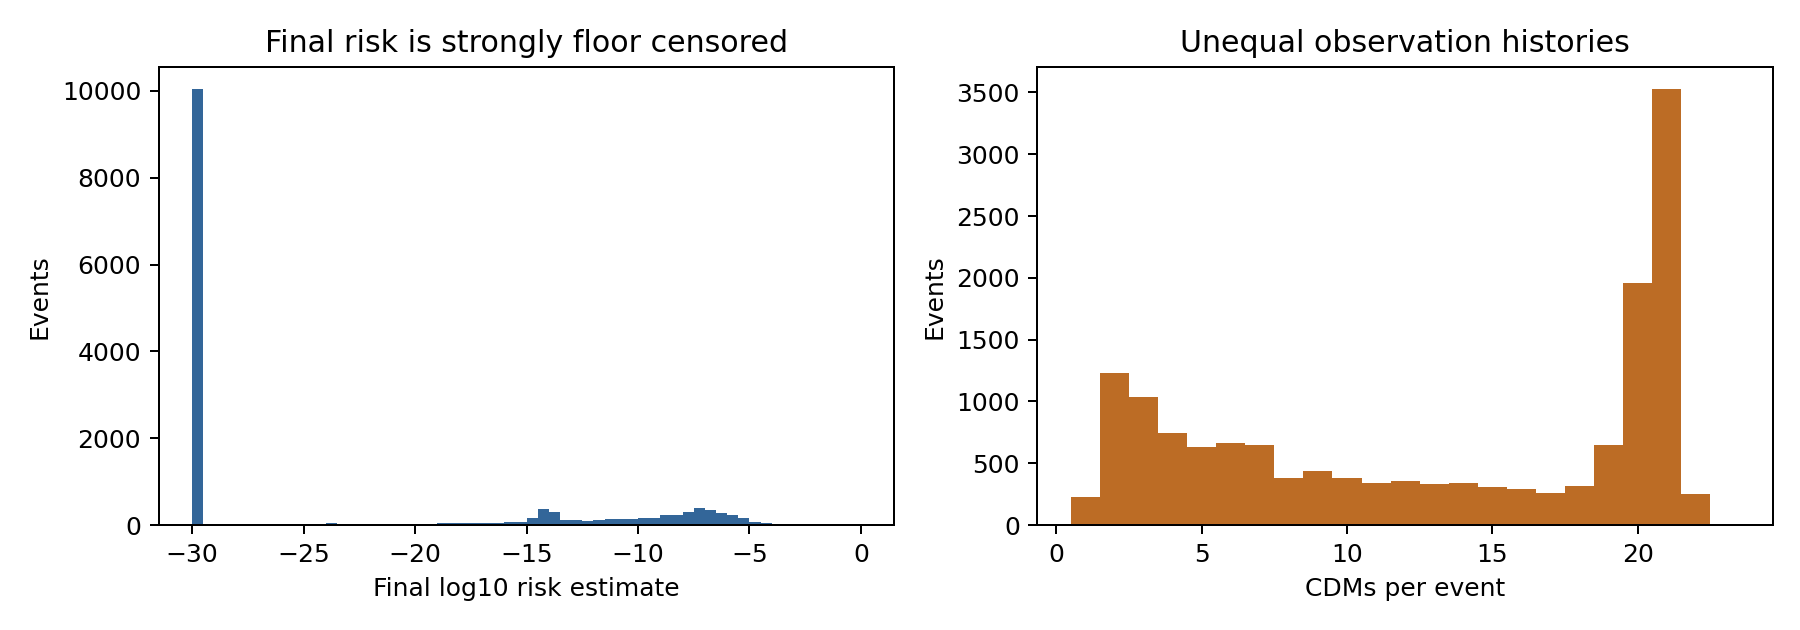
\includegraphics[width=.93\linewidth]{distributions.png}\caption{The final risk distribution has a large point mass at $-30$; event histories vary from one to 23 CDMs.}\end{figure}
The chaser radar cross-section estimate is missing in 32.1\% of CDMs. A cluster of chaser covariance entries is missing in 5.6\%. Risk itself has no missing values. These patterns plausibly depend on object type and observation process, so missing completely at random is not a defensible default. A logistic missingness model including current risk, miss distance, object type and target altitude band was fitted to diagnose observed dependence; it cannot test whether missingness depends on the unobserved value itself.

For the one coefficient involving chaser radar cross section, five chained-equation imputations were combined with Rubin's variance formula under conditional missing at random. The pooled effect estimate was small and its 95\% interval crossed zero (see machine-readable table). Complete-case and imputed estimates are shown side by side. This is a sensitivity exercise, not proof that the missing-at-random assumption holds; the main predictive feature set excludes radar cross section. Numerical imputation for other selected predictors is performed separately inside each fitted pipeline, with a missing-indicator channel supplied to tree models.

The target perigee spans roughly 273--825 km in this archive. Consequently all monitored target spacecraft in this release are in low Earth orbit. Analyses use low ($<550$ km), middle (550--700 km) and upper ($>700$ km) LEO bands. The data do not support a LEO-versus-GEO comparison. Median final-minus-initial capped risk is $-2.67$ log$_{10}$ units (event-bootstrap 95\% interval $[-2.83,-2.48]$) among near-TCA events. The median log$_{10}$ ratio of final to initial position-sigma norm is $-1.43$ (interval $[-1.45,-1.42]$). Risk and uncertainty revisions have Spearman $\rho=0.338$ after complete pairs. This is consistent with correlated refinement of geometry and covariance, not a causal effect of reducing sigma.
\clearpage
\section{E1: frequentist risk evolution and diagnostics}
A training-event OLS baseline at 72 hours models capped final log risk as a function of centred current risk, log miss distance, centred log position uncertainty, log observation count, available CDM count, altitude-band indicators and a current-risk-by-uncertainty interaction. Under a Gaussian working likelihood, OLS equals the maximum-likelihood coefficient estimator. HC3 sandwich standard errors address observed heteroscedasticity for coefficient intervals; they do not make the conditional mean specification correct. The model has $R^2=0.196$ on 5,869 training events, AIC 24,266 and BIC 24,326. These criteria compare only likelihood models fitted to the \emph{same} capped outcome and observations.

At mean log uncertainty, one additional unit of current log risk is associated with a $0.230$ increase in final capped log risk (HC3 95\% CI 0.206--0.255). The unadjusted slope is $0.259$; its attenuation after geometry, uncertainty and observation adjustment illustrates measured confounding. Log miss distance has coefficient $-0.204$ (CI $-0.254$ to $-0.154$). The risk-by-uncertainty interaction has a likelihood-ratio statistic $0.976$ on one degree of freedom ($p=0.323$), so this particular linear interaction is not established. Many observed features are physically and algorithmically related to the calculated risk, making all coefficients associational.

A binomial-logit GLM for final risk at least $10^{-5}$ has 43 positives among the 72-hour training events. Its altitude-band extension over a nested model has likelihood-ratio statistic 2.630 on two degrees of freedom ($p=0.268$). Sparse positives make Wald intervals and odds ratios sensitive to specification; the saved coefficient table includes robust intervals. The GLM represents a probability of a future \emph{risk category}, not a physical collision probability.

Diagnostics argue against overinterpreting the OLS fit. Breusch--Pagan and Jarque--Bera tests both reject the classical constant-variance/normal-residual assumptions at machine precision; a RESET check has $p\approx3\times10^{-48}$. About 8.0\% of rows exceed Cook's $4/n$ heuristic. Centring the interaction reduces unnecessary collinearity, while substantial predictor dependence remains. These findings motivate the nonlinear and robust distributional alternatives below.
\clearpage
\section{E2: longitudinal heterogeneity and hierarchical inference}
A within-event model asks whether successive reports share an encounter-specific level beyond measured time, miss distance and uncertainty. On a fixed random sample of 220 events (3,135 CDMs), a Gaussian random-intercept mixed model yields random-intercept variance 7.50 and residual variance 3.95, giving intraclass correlation
\begin{equation}
\mathrm{ICC}=\frac{\tau_{\rm event}^2}{\tau_{\rm event}^2+\sigma^2}=0.655.
\end{equation}
This large conditional event component supports modelling encounters as dependent series. The mixed-model maximum-likelihood AIC is 13,914 and BIC 13,950 for this selected sample. Its Gaussian/capped outcome is a working model, so the ICC is descriptive and should not be extrapolated unchanged to all events.

A focused Bayesian hierarchy models CDMs with reported log risk above $-15$ and a within-event nonfloor risk range no greater than five log units. The restriction removes the exact floor and the abrupt-revision events that produced multimodal Student-$t$ random-effect posteriors. For observation $j$ of event $i$, standardized response $z_{ij}=(r_{ij}+10)/5$ follows
\begin{align}
 z_{ij} &\sim N(\alpha+\beta\,\widetilde t_{ij}+u_i,\sigma^2),\\
 (u_1,\ldots,u_I)&\sim\mathrm{ZeroSumNormal}(0,\tau_e^2),
\end{align}
where $\widetilde t$ is standardized TCA lead time. The 100-event, 616-CDM demonstration spans 11 missions, but mission effects are omitted because satellite identity is unavailable and mission/event effects were not separately identifiable in exploratory fits. Four NUTS chains with 500 tune and 500 posterior draws yield posterior mean event scale $0.620$ (95\% HDI 0.531--0.713), maximum $\hat R=1.01$, minimum bulk ESS 823 and zero divergences. In-sample 90\% posterior predictive coverage is 93.2\%. The Gaussian likelihood is a working approximation only for this stable, nonfloor subset; it is not imposed on the full archive.

These random effects describe repeat observations from known, stable events. Predicting a \emph{new} event requires integrating over an unseen $u_i$, and abrupt revisions remain a failure mode. We therefore do not claim that the hierarchy improves new-event uncertainty without blocked validation. Satellite-level effects cannot be identified because satellite identity is not released.
\clearpage
\section{Bayesian continuous-risk model: priors, NUTS and checks}
For a focused event-level analysis, 761 eligible 72-hour training events with final log risk above $-15$ are modelled. This conditional subset excludes the exact floor mass; its results cannot be compared directly with full-cohort capped-risk scores. Predictor columns (current risk, log miss distance, log sigma norm, CDM count, target perigee) are standardized on this training subset. For $z_i=(r_{i,F}+10)/5$,
\begin{align}
 z_i&\sim t_{\nu}(\alpha+x_i^{\mathsf T}\beta,\sigma),\\
 \alpha&\sim N(0,2^2),\quad \beta_k\sim N(0,s^2),\quad \sigma\sim\mathrm{HalfNormal}(2),\quad \nu-2\sim\mathrm{Exponential}(0.1),
\end{align}
with $s=0.5$ and $2$ as a prior-scale sensitivity pair. PyMC with NumPyro NUTS ran two chains of 300 tune and 300 posterior iterations per prior. Posterior summaries are in the accompanying CSVs; for $s=2$, standardized current-risk coefficient is $0.696$ (95\% HDI 0.676--0.713), while log sigma is $-0.031$ ($-0.042$ to $-0.021$). These are conditional associations on the standardized outcome and selected nonfloor cohort.

Both fits have maximum $\hat R=1.01$, minimum bulk ESS above 380 and zero divergences. Their expected log pointwise predictive densities from event-level PSIS-LOO are $-296.67$ and $-296.71$ for the narrower and wider priors; WAIC values are $-296.63$ and $-296.67$. No Pareto $k$ exceeds 0.7. The difference in LOO is only 0.04, far too small to assert one prior is superior. Each row is a distinct event, so event-level PSIS-LOO has the appropriate independent unit here. WAIC and LOO are not computed on conditional random-effect CDMs as though rows were independent.

Posterior predictive 90\% intervals cover only about 77\% of the training observations, despite acceptable sampler diagnostics. This is a model-check failure: convergence is not calibration. Conditional held-out results are \BayesCondMAE\ MAE on \BayesCondN\ nonfloor test events, with observed 90\% interval coverage of \BayesCondCoverage. On the same 761/205 conditional train/test events, a focused ridge model has MAE 1.725 and XGBoost 1.606; the Bayesian posterior mean reaches 1.463. This is evidence for that selected continuous component only, not a deployable full-cohort advantage. The undercoverage is consistent with misspecified conditional shape or truncation at $-15$; a full hurdle/censoring model is a priority for future work.
\clearpage
\section{E3: prediction horizons on comparable encounters}
\begin{figure}[h]\centering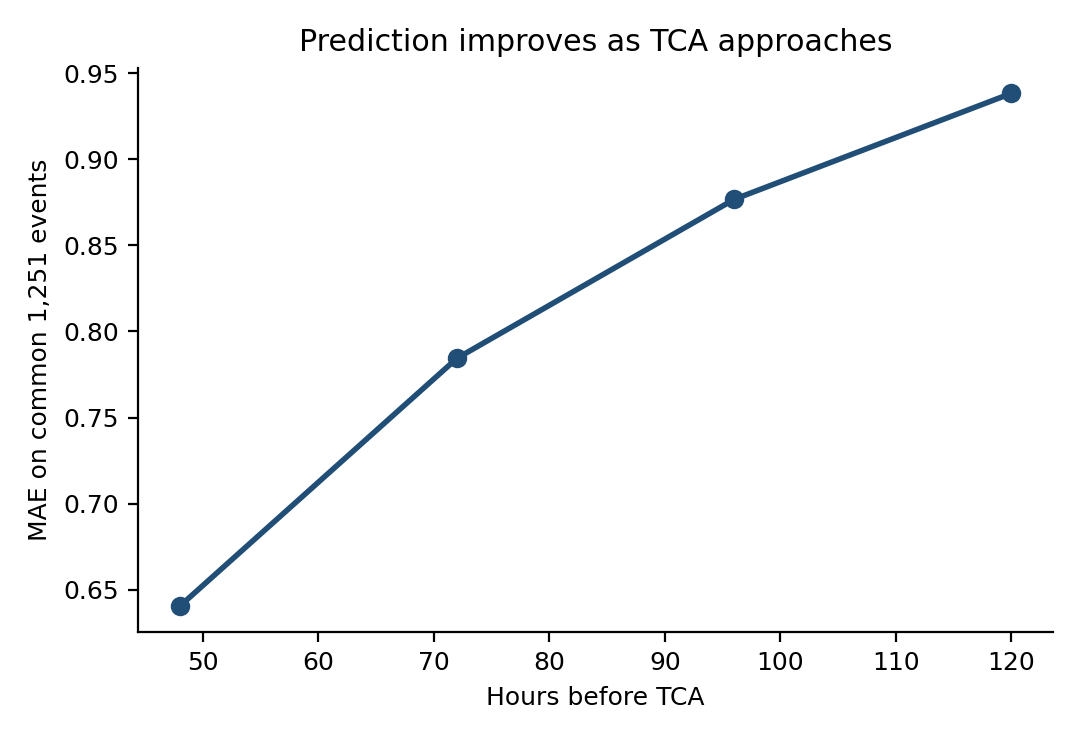
\includegraphics[width=.78\linewidth]{paired_horizons.png}\caption{XGBoost evaluation on exactly the same 1,251 events at all four cutoffs.}\end{figure}
The common-cohort experiment isolates lead-time information from changing eligibility. XGBoost MAE on capped log risk is 0.938 at 120 hours, 0.877 at 96, 0.784 at 72 and 0.640 at 48. The direction is monotone, consistent with later CDMs improving final-estimate forecasting. It does not imply that waiting is always operationally preferable: an avoidance decision needs lead time, and false alarms carry costs.

Separate full-eligible test cohorts grow from 1,251 to 1,564 events as the cutoff moves from 120 to 48 hours. Their XGBoost MAEs are 0.938, 0.907, 0.846 and 0.724, respectively. Because these samples differ, the full-cohort trend confounds time and case mix; the paired result above is the primary horizon comparison. The risk floor also means a single absolute-error average rewards accurate identification of negligible-risk events. We therefore report the threshold task alongside regression and do not infer warning utility from MAE alone.

The horizon rule uses the latest CDM satisfying $t\geq h/24$ days. A message at 49 hours contributes to the 48-hour snapshot, while a message at 47 hours does not. An event with no earlier message cannot enter that horizon. No interpolation or future-CDM borrowing fills gaps. Observation count and history span are included as predictors; subgroup results test the consequences of sparse histories rather than treating missing earlier CDMs as random omission.
\clearpage
\section{E4: frequentist, Bayesian, ML and DL comparison}
\begin{figure}[h]\centering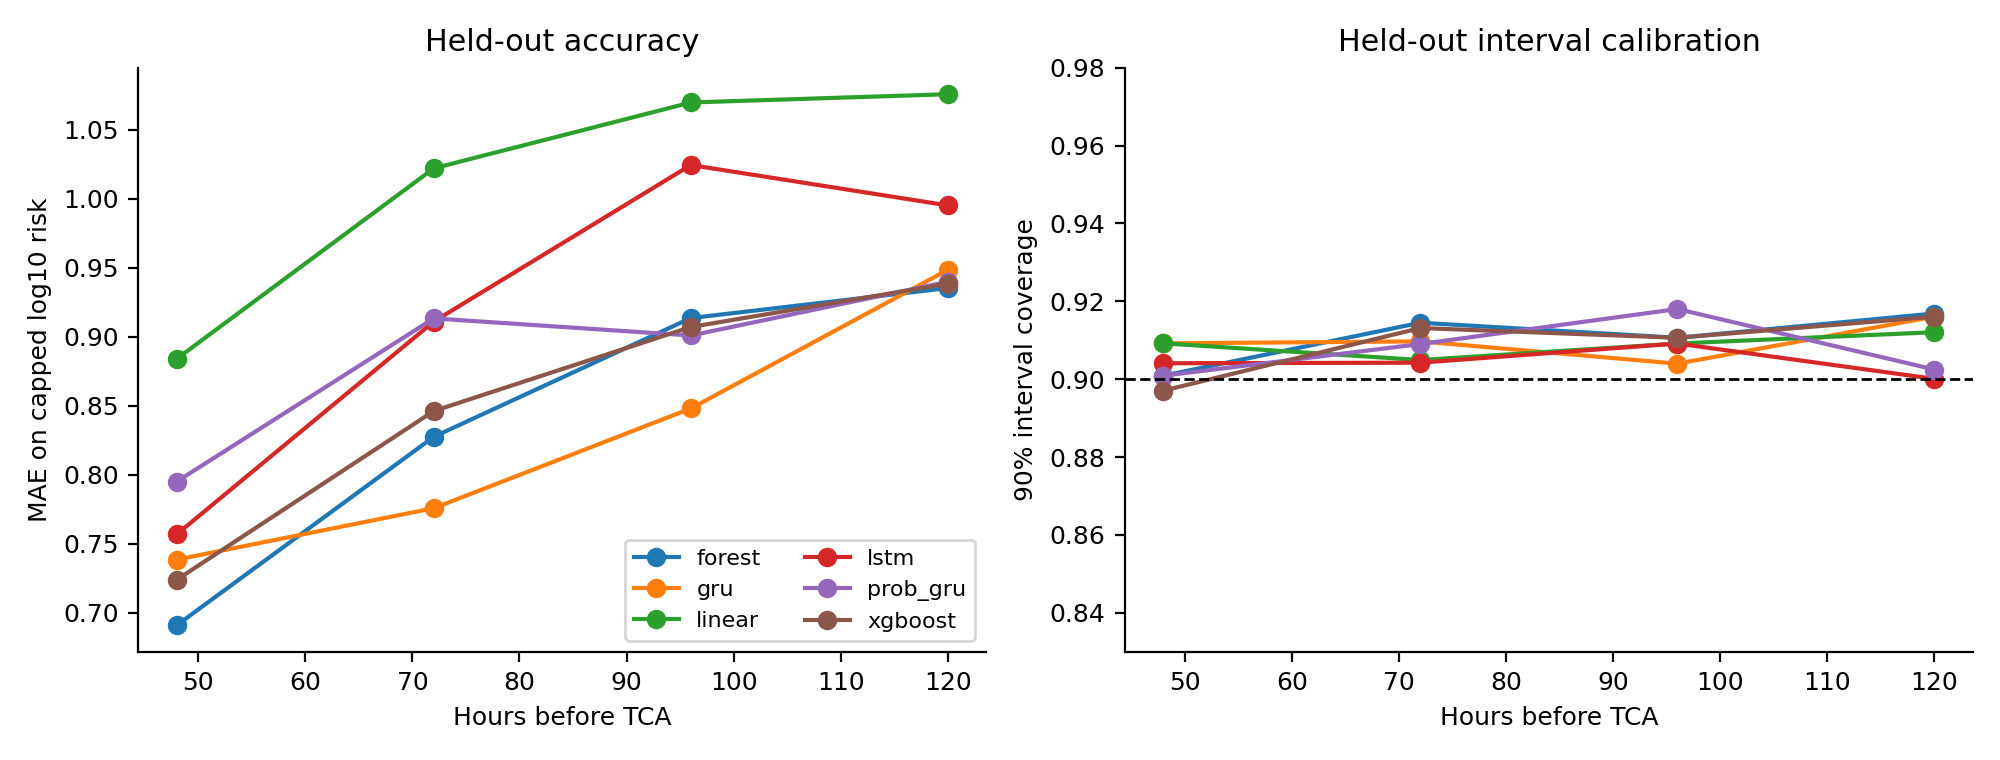
\includegraphics[width=.95\linewidth]{model_comparison.png}\caption{Held-out full-cohort MAE and interval coverage. Lower MAE is better; the dashed coverage line marks nominal 90\%.}\end{figure}
At 72 hours, linear regression MAE is 1.022, random forest 0.828, XGBoost 0.846, GRU 0.776, LSTM 0.911 and probabilistic GRU 0.913 log$_{10}$ units. At 48 hours, the forest is best among these models at 0.691, while GRU reaches 0.739. The event-bootstrap XGBoost-minus-linear MAE difference at 72 hours is $-0.176$ (95\% interval $[-0.205,-0.144]$). GRU-minus-forest is $-0.052$ ($[-0.085,-0.019]$) at 72 hours but $+0.048$ ($[0.014,0.080]$) at 48 hours. Thus complexity has horizon-dependent value; neither neural networks nor boosted trees dominate throughout.

The approaches answer related but distinct questions. Frequentist OLS and GLM deliver transparent conditional associations, tests and confidence intervals but fail several working assumptions here. Bayesian regression supplies posterior distributions and prior checks for the nonfloor component, attaining conditional-test MAE 1.463 versus 1.725 for a matched ridge and 1.606 for a matched XGBoost; its observed 90\% coverage is only 79.0\%. Full-cohort ML and DL scores below cannot be ranked directly against that selected Bayesian component.\par\medskip

The tree configurations are intentionally modest: shallow XGBoost, 120--150-tree forests, median-imputed shared features. A three-fold event-grouped training-only grid tests nearby settings at 72 hours: forest leaf sizes 5 and 8 both yield MAE about 0.880; XGBoost depths 2, 3 and 4 yield 0.934, 0.902 and 0.892. The 0.010 gap between depths 3 and 4 is smaller than the across-fold standard deviation, so the held-out comparison retains depth 3 as a compact fixed configuration. GRU and LSTM use a single 24-unit recurrent layer, padded variable-length histories, explicit elapsed-time gaps and missingness masks. The probabilistic GRU emits Gaussian mean and scale; its Gaussian log score and interval calibration are assessed separately. Ten-epoch maximum training with validation monitoring limits overfitting. Native XGBoost SHAP contributions on a 72-hour test sample rank current risk, risk revision, chaser observation count and miss distance highest; they describe the fitted model and do not establish causal effects. Hyperparameter exploration is deliberately narrow, so this is a comparison of reproducible compact implementations, not an exhaustive leaderboard.
\clearpage
\section{E5: interval and probability calibration}
For each point predictor $\hat y$, a separate calibration partition supplies absolute residuals $e_i=|y_i-\hat y_i|$. The split-conformal 90\% interval is $[\hat y-q,\hat y+q]$, where $q$ is the finite-sample $\lceil(n_{\rm cal}+1)0.9\rceil/n_{\rm cal}$ residual quantile. Under exchangeability of calibration and test events, marginal coverage is at least approximately 90\%; it is not guaranteed conditional on a particular altitude band, risk level or mission. Observed coverage for the models is about 89.7--91.8\% across tested horizons. At 72 hours, XGBoost covers 91.3\% with mean width 6.00 capped-log units, while the forest covers 91.5\% with width 6.42. These wide intervals reflect the difficulty of forecasting individual revisions.

The probabilistic GRU has a Gaussian likelihood and reports Gaussian negative log likelihood after a scale adjustment on calibration events. At 72 hours its held-out NLL is 1.756 and 90\% interval coverage 90.9\%, with mean width 3.83. Its MAE and RMSE are worse than the point GRU, so nominal coverage alone is not sufficient. A Gaussian density on a capped target is misspecified at the point mass; the log score must be read with this caveat. Bayesian conditional intervals cover only roughly 77\% in sample and \BayesCondCoverage\ in the nonfloor test subset. The two likelihoods and target populations differ, so their raw interval widths should not be ranked as if they were identical predictive problems.

For warnings, Brier score and Bernoulli log loss are proper probability scores. Classifier probabilities receive an intercept recalibration on the calibration partition. A threshold is then chosen from that same partition under an approximately 5\% false-positive-rate constraint, favoring recall. The small number of positive calibration examples makes the threshold unstable. Reliability bins and event-bootstrap uncertainty therefore accompany the warning table. A false-positive rate of 5\% still generates many alerts when the base rate is below 1\%.
\clearpage
\section{E6 and E7: sparse histories and early warning}
At 72 hours, the XGBoost regression MAE is 1.139 on 218 test events with only one to three prior CDMs, versus 0.795 on 1,244 events with at least four. Only one high-final-risk event occurs in the sparse subgroup, so its warning recall is not estimable with useful precision. Observation count may be a marker of surveillance process and encounter severity; the subgroup difference is associational, not the effect of supplying more CDMs experimentally.

The $10^{-5}$ warning objective is rare. At 72 hours, the XGBoost rule labels 73 of 1,462 test events: 4 true warnings and 69 false alarms. Recall is 57.1\%, precision 5.48\%, false-positive rate 4.74\%; three high-risk final estimates are missed. Event-bootstrap 95\% intervals are 1.2--10.8\% for precision and 14--100\% for recall. At 48 hours, 7 of 9 high-risk events are caught, with 76 false alarms and 8.4\% precision. At 120 hours, only 3 of 6 are caught, with 79 false alarms and 3.7\% precision. The logistic baseline has similar or slightly better precision at 72 hours. A deployment threshold should be chosen using mission-specific loss and a representative base rate, not the competition's enriched prevalence.

\begin{figure}[h]\centering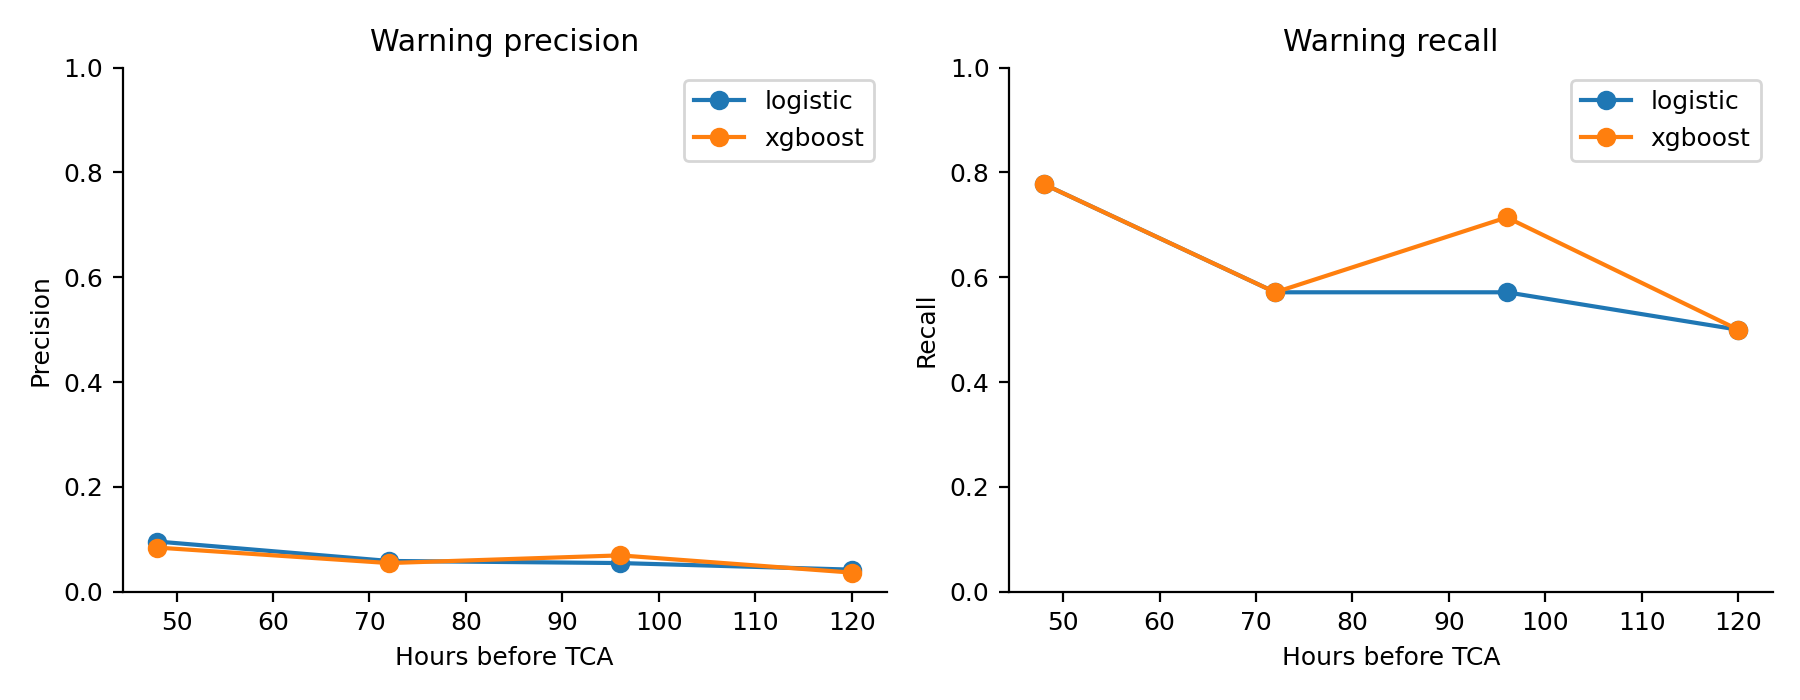
\includegraphics[width=.84\linewidth]{warnings.png}\caption{Precision and recall by lead time on changing eligible cohorts; small positive counts make lines noisy.}\end{figure}
\clearpage
\section{E8: robustness, selection and limits of inference}
The most consequential distribution shift is visible in the official competition split. In the separately fitted 48-hour official experiment, 8,293 training events satisfy the near-TCA eligibility rule and only 0.277\% exceed $10^{-5}$; 2,167 released test events have a 2.584\% high-risk rate. The test enrichment is about 9.3-fold. Selecting the top 5\% of official-test scores yields 35.8\% precision and 69.6\% recall, values that must not be transported to the natural-prevalence archive cohort. The official regression MAE is 1.058, also reflecting a different selected test population.

Within the raw 72-hour test cohort, XGBoost MAE varies by target altitude band: 0.658 on 300 low-LEO events, 0.806 on 735 middle-LEO events and 1.047 on 427 upper-LEO events. These bands differ in mission mix, geometry and data quality; no altitude causal effect is identified. A ridge model trained without the most common mission has MAE 0.919 on 244 test events from that mission, a limited transfer check. Exact satellite and date dependence cannot be examined. The Bayesian event-level model's two prior scales yield virtually identical PSIS-LOO scores; that specific prior perturbation does not remedy posterior undercoverage. The imputed radar-cross-section coefficient remains uncertain and is not used as a decisive predictor.

Several modelling risks remain. The $-15$ cap treats values between $-30$ and $-15$ as equal; a full hurdle or censored model could improve coherent density forecasts. The 72-hour OLS residual checks show misspecification. Rare warnings yield very wide intervals and sensitivity to a few events. Split conformal coverage relies on exchangeability and is marginal, whereas mission and epoch shift could break it. No true collision outcomes are observed, and risk estimates are derived from some of the same geometry and covariance inputs used as predictors. These limitations preclude causal language and operational validation claims.
\clearpage
\section{Synthesis and conclusion}
The principal statistical result is that uncertainty must be judged empirically. Hierarchical models reveal strong encounter-level dependence (frequentist ICC 0.655; Bayesian event scale 0.620), but a converged Bayesian conditional regression still undercovers. In contrast, simple split-conformal calibration of held-out point-model residuals attains near-nominal marginal coverage, albeit with very wide intervals. This does not prove conformal prediction solves mission transfer, high-risk conditional calibration or physical collision uncertainty; it answers a narrower event-exchangeable archive question.

More recent CDMs improve final-risk forecast accuracy on the same events, but usable warning lead time trades against false alarms and missed high-risk estimates. Tree models are consistently stronger than the linear full-cohort baseline. A small GRU adds information at 72 and 96 hours but loses to a forest at 48 hours; extra model complexity is justified only when the horizon and validation population support it. Bayesian hierarchy provides interpretable partial pooling for observed event histories, while its new-event predictive advantage remains unverified. The model class preferred for admissions-quality statistical reasoning is therefore question-specific: regression and GLMs for transparent associations, mixed/hierarchical models for dependence, and calibrated ensembles or sequences for forecasting.

\textbf{Answer.} Statistically principled uncertainty modelling improves the \emph{assessment} when it exposes dependence, checks assumptions and calibrates intervals on untouched events. This study does not find evidence that the fitted Bayesian predictive intervals themselves improve reliability. Simpler models remain valuable interpretive baselines; forests, boosting and occasionally GRUs improve point accuracy. Future work should fit a joint hurdle/censoring model, validate on genuinely later missions with known spacecraft identities, use grouped cross-validation for model selection, and evaluate mission-specific decision losses on a deployment-representative sample.

\section*{References}
\begin{thebibliography}{9}
\bibitem{esa-data} Uriot, T., Izzo, D., Martinez-Heras, J., Letizia, F., Siminski, J. and Merz, K. (2021). \emph{Collision Avoidance Challenge dataset}. Zenodo. DOI: \href{https://doi.org/10.5281/zenodo.4463683}{10.5281/zenodo.4463683}.
\bibitem{esa-doc} European Space Agency (2019). \emph{Collision Avoidance Challenge: Data and column descriptions}. \url{https://kelvins.esa.int/collision-avoidance-challenge/data/}.
\bibitem{uriot2020} Uriot, T. et al. (2020). \emph{Spacecraft Collision Avoidance Challenge: Design and Results of a Machine Learning Competition}. arXiv:2008.03069. \url{https://arxiv.org/pdf/2008.03069.pdf}.
\end{thebibliography}
\clearpage
\section*{Appendix: statistical component and experiment audit}
\small
\begin{tabular}{>{\raggedright\arraybackslash}p{.27\linewidth}>{\raggedright\arraybackslash}p{.65\linewidth}}
\toprule
Component & Implementation and diagnostic role\\\midrule
Linear regression, MLE & 72-hour OLS on capped final risk; likelihood and HC3 interval estimates.\\
GLM, MLE & Binomial logit for final risk $\geq10^{-5}$; robust coefficient table.\\
Likelihood-ratio/Wald tests & Nested interaction and altitude-band tests; HC3 Wald tests in coefficient tables.\\
Confidence intervals & HC3 coefficients, event-bootstrap median revisions and paired MAE differences.\\
Mixed effects & Event random intercept on repeated CDMs; variance components and ICC.\\
Bayesian linear regression & Student-$t$ continuous nonfloor regression with explicit priors and posterior HDIs.\\
Bayesian hierarchy & Event random intercepts on a stable nonfloor supplementary subset.\\
Hamiltonian Monte Carlo & PyMC/NumPyro NUTS, two chains; $\hat R$, ESS and divergences saved.\\
Posterior predictive checks & In-sample interval coverage, plus held-out conditional event-level coverage.\\
AIC/BIC & Gaussian OLS and mixed likelihood; GLM AIC/BIC from binomial likelihood.\\
Cross-validation & Three-fold event-grouped training-only grid, plus disjoint validation/calibration/test and official selection check.\\
WAIC and PSIS-LOO & Event-level continuous Bayesian regression; Pareto-$k$ diagnostics.\\
Bootstrap intervals & Events resampled for revisions, warning precision/recall and paired model gaps.\\
Calibration & Split-conformal regression coverage, classifier Brier/log loss, reliability bins.\\
Confounding and interaction & Unadjusted/adjusted risk slope; risk-by-uncertainty interaction.\\
Diagnostics and priors & Residual, heteroscedasticity, RESET, influence, VIF, PPC and prior scale.\\
Missing-data mechanism & Missingness profiling and five-imputation conditional-MAR sensitivity.\\
\bottomrule
\end{tabular}

\vspace{0.4cm}
\textbf{Reproduction.} Fixed seeds appear in each script. The exact environment is frozen in \texttt{requirements.lock}. Source tables, test predictions, figures and posterior chains are saved in \texttt{outputs/}. The leakage checks in \texttt{08\_validate.py} passed on 37,622 horizon snapshots. The PDF was built from this editable \LaTeX{} source.
\end{document}
